\documentclass{article}

\usepackage[final]{nips_2016}

\usepackage[utf8]{inputenc}
\usepackage[T1]{fontenc}
\usepackage{hyperref}
\usepackage{url}
\usepackage{booktabs}
\usepackage{amsfonts}
\usepackage{nicefrac}
\usepackage{microtype}
\usepackage{graphicx}
\usepackage{makecell}
\usepackage{algorithm}
\usepackage{algpseudocode}
\usepackage{bm}
\usepackage{amsmath}
\usepackage{makecell}
\usepackage{subcaption}

\title{Enhancing Multiple Myeloma Cell Segmentation through Physical Image Transformations}

\author{%
  Archit Kaila\\
  Artificial Intelligence\\
  Duke University\\
  Durham, NC 27705\\
  \texttt{archit.kaila@duke.edu} \\
  \And
  Shen Juin Lee \\
  Artificial Intelligence\\
  Duke University\\
  Durham, NC 27705\\
  \texttt{shenjuin.lee@duke.edu} \\
  \And
  Shrey Gupta\\
  Artificial Intelligence\\
  Duke University\\
  Durham, NC 27705\\
  \texttt{s.gupta@duke.edu} \\
}

\begin{document}
% \nipsfinalcopy is no longer used

\maketitle

\begin{abstract}
Multiple Myeloma (MM) is a type of blood cancer that is caused by the abnormal expansion of plasma cells in the bone marrow. Recently, there have been efforts to develop computer-assisted diagnostic tools for MM through artificial intelligence and image processing. These tools require the capture and normalization of images, as well as the segmentation and classification of cells as malignant or healthy. However, the segmentation of plasma cells in MM is particularly challenging due to various factors, such as varying amounts of nucleus and cytoplasm in each cell, the presence of clustered cells which leads to the cytoplasm of two cells touching each other, and the possibility of unstained cells or cytoplasm that blends into the background. We aim to enhance the accuracy of segmentation by applying physical imaging transformations to the raw microscopic images.
\end{abstract}

\section{Introduction}

Cancer is a disease that occurs when the cells in the body start to proliferate uncontrollably and spread to the surrounding tissues. Normal cells in the body grow, divide and die, but cancer cells continue to divide and form new abnormal cells. Multiple Myeloma is a type of blood cancer that arises from plasma cells in the bone marrow. In Multiple Myeloma, plasma cells grow in the bone marrow in a way that there is no space for normal red blood cells, white blood cells and platelets. The definitive diagnosis of Multiple Myeloma is usually done through manual analysis of aspirate slide images, which can show the histology and morphological features of Multiple Myeloma cells. Based on the count and features of plasma cells in bone marrow, the presence or absence of Multiple Myeloma cells can be inferred. However, manual inspection of stained slide images is a time-consuming process that is prone to variations in methdology and observation, despite being considered the gold standard for Multiple Myeloma diagnosis.

Advanced digital image processing techniques, such as object detection and segmentation, can help overcome these limitations by automating the abnormal plasma cell detection process. By combining these techniques with expert pathologist decision-making, it may be possible to reduce diagnosis time and alleviate the workload of pathologists. The primary objective of developing an automated diagnostic tool for Multiple Myeloma is to perform accurate segmentation of cells, which is a challenging task due to the variety of possible scenarios. The SegPC-2021 Challenge [1] aimed to address this issue by providing bone marrow aspirate slide images from Multiple Myeloma patients. Segmentation of plasma cells in these images is complicated due to several factors, such as the presence of cell clusters, cells with varying nucleus and cytoplasm sizes, and difficulty in distinguishing cells that are touching. Additionally, the staining process used in preparing the slides may not be perfect, resulting in cells that are not stained or cells with cytoplasm that blends with the background color. The task becomes even more challenging due to the use of computer-generated labels, which may contain inconsistencies and noise.

Research on automated cell segmentation in microscopic images has been ongoing for many years. However, recent advancements in deep learning have led to significant breakthroughs in this field. U-Net, a fully convolutional neural network architecture, has demonstrated remarkable results in cell segmentation and tracking challenges. Similarly, Mask R-CNN [2], a universal approach to instance segmentation, has been adapted to different domains, including cell nucleus segmentation. Instead of purely optimizing deep learning model architectures, it is hypothesized that optimizing imaging systems could improve the performance of instance segmentation. However, constructing and implementing different imaging systems can be both costly and time-consuming. Simulating various physical imaging systems and identifying the best performing one, on the other hand, is a more feasible approach. The purpose of this study is to devise an improved method for the detection of Multiple Myeloma cells in microscopic images by utilizing existing object detection and instance segmentation algorithms and augmenting them with various image transformation techniques, thereby simulating various physical imaging systems.

\section{Related Work}
Previous research has been conducted in attempt to identify Multiple Myeloma cells using deep learning based methods.

In Gupta A et al [3], the paper discussed multiple approaches to tackle the challenge on segmentation of Multiple Myeloma cells on microscopic images. The top solution combined three instance segmentation models with three convolutional feature extractors, extensive image augmentation, and a custom model ensemble strategy. It utilized a post-processing step to pair corresponding instances of nuclei and cytoplasm together, using an auxiliary whole-cell class. The second-placed solution used a two-stage approach where the first stage consisted of extraction of possible nucleus instances using a U-Net and the second stage relied on dilated convolution and attention mechanism using Attention Deeplabv3+ for cytoplasm segmentation.

Paing MP et al [4] explored instance segmentation of Multiple Myeloma cells using Mask Region-based Convolutional Neural Network (R-CNN) models. They applied deep-wise augmentation, a deep learning-based data augmentation method to increase the performance of their models. However, none of these previous works incorporated physical imaging techniques to enhance the identification of Multiple Myeloma cells.

\section{Methodology}
\subsection{Data Sources \& Processing}
For this work, we used the SegPC-2021 challenge dataset, a medical imaging challenge on on "Segmentation of Multiple Myeloma Plasma Cells in Microscopic Images (SegPC-2021)" organized at the IEEE International Symposium on Biomedical Imaging (ISBI), 2021, France. The dataset was obtained from patients diagnosed or treated for Multiple Myeloma (MM) at AIIMS, New Delhi, India. Microscopic images were captured from bone marrow aspirate slides using two cameras: 1. Olympus camera with an image size of 2040x1536 pixels and 2. Nikon camera with an image size of 1920x2560 pixels. The images were captured using a stain color normalization technique to reduce the color variations in the images and were divided into three sets:
\begin{enumerate}
  \item Train (298 images)
  \item Validation (200 images)
  \item Test (277 images)
\end{enumerate}
The Ground Truth (GT) values were provided for the train and validation sets, but not for the test set. These were provided in form of a mask where each mask is an image with a single segmented Multiple Myeloma cell. The background of the mask had a pixel value of 0, the nucleus of the cell was represented by a pixel value of 40, and the cytoplasm of the cell was represented by a pixel value of 20. The masks were of the same size as the original images.

To use the dataset in our experiments, we first resized the images to the dimensions of 1080x1440 pixels since the desired outputs were expected in this size and then converted the given ground truth image masks into Common Objects in Context (COCO) annotation format. The COCO annotation format is a JSON file that contains the image ID, image size, and the bounding box and segmentation mask coordinates of the nucleus and cytoplasm of the cell. The bounding box coordinates are provided in the form of the top-left and bottom-right coordinates of the bounding box. The segmentation mask coordinates represent the polygonized contour of the Multiple Myeloma cells. The COCO annotation format is used in the Detectron2 [5] library for object detection and instance segmentation. The Detectron2 library was used for training and evaluating the Mask R-CNN model in our experiments.

\subsection{Physical Image Transformations}

The segmentation of Multiple Myeloma cells can be challenging due to their morphological heterogeneity and similarities with normal plasma cells. In the dataset, there are instances where the cells can overlap, or where the nucleus covers much of the foreground, hiding the cytoplasm in the background. To improve the precision of segmenting the nucleus and cytoplasm of Multiple Myeloma cells, various physical image transformations were applied to pre-process the images in specific ways. These transformations could enhance image contrast, reduce noise, improve edge detection, and extract meaningful features, potentially leading to more accurate segmentation results. In this section, we describe the physical image transformations that we applied to the raw images in attempt to improve the segmentation of Multiple Myeloma cells.

\subsubsection{Illumination Simulation}
In this image transformation, we attempted to simulate the illumination of a sample by a microscope. We assumed that the microscope had 12 LEDs in a rectangular array at the bottom and mimicked the absorption of light waves by the sample and the subsequent passage of light through the microscope lens after an optical phase shift. The illumination layer featured trainable weights that took a weighted sum of all twelve resulting images and combined them into a single channel image, which was then fed to the rest of the model to segment the nucleus and cytoplasm of Multiple Myeloma cells. The rationale behind this illumination layer was to improve segmentation performance by providing a more realistic and consistent illumination across a microscope slide. Furthermore, this could minimize the impact of shadows that could confound the identification of Multiple Myeloma cells amidst surrounding cells. Shadows could form due to non-uniform illumination or light obstruction by nearby structures, resulting in darker areas within the image. By simulating the illumination of the sample, we can reduce the impact of shadows and improve the accuracy of segmentation.

\subsubsection{Contrast Normalization}
The contrast of a sample could be a critical factor for accurate segmentation. By enhancing the contrast between Multiple Myeloma cells and surrounding cells, we aimed to improve the accuracy of segmentation algorithms that rely on pixel intensity variations. This feature may be particularly relevant when dealing with images of low contrast or high noise levels. In microscopic images, the contrast between Multiple Myeloma cells and surrounding cells can differ due to variations in illumination or staining methdology. This can make it challenging for segmentation algorithms to distinguish Multiple Myeloma cells from other cells. Contrast normalization is a widely used image transformation technique that aims to improve the contrast of an image. It works by rescaling the pixel values of an image so that they fall within a specified range. This can help to make Multiple Myeloma cells more distinguishable from red blood cells or other cells, which may have similar pixel intensity values.

\begin{figure}
  \centering
  \begin{minipage}{.5\textwidth}
    \centering
    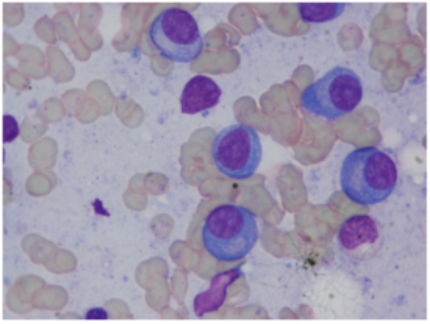
\includegraphics[width=.5\linewidth]{1.png}
    \captionof{figure}{Original Image}
  \end{minipage}%
  \begin{minipage}{.4\textwidth}
    \centering
    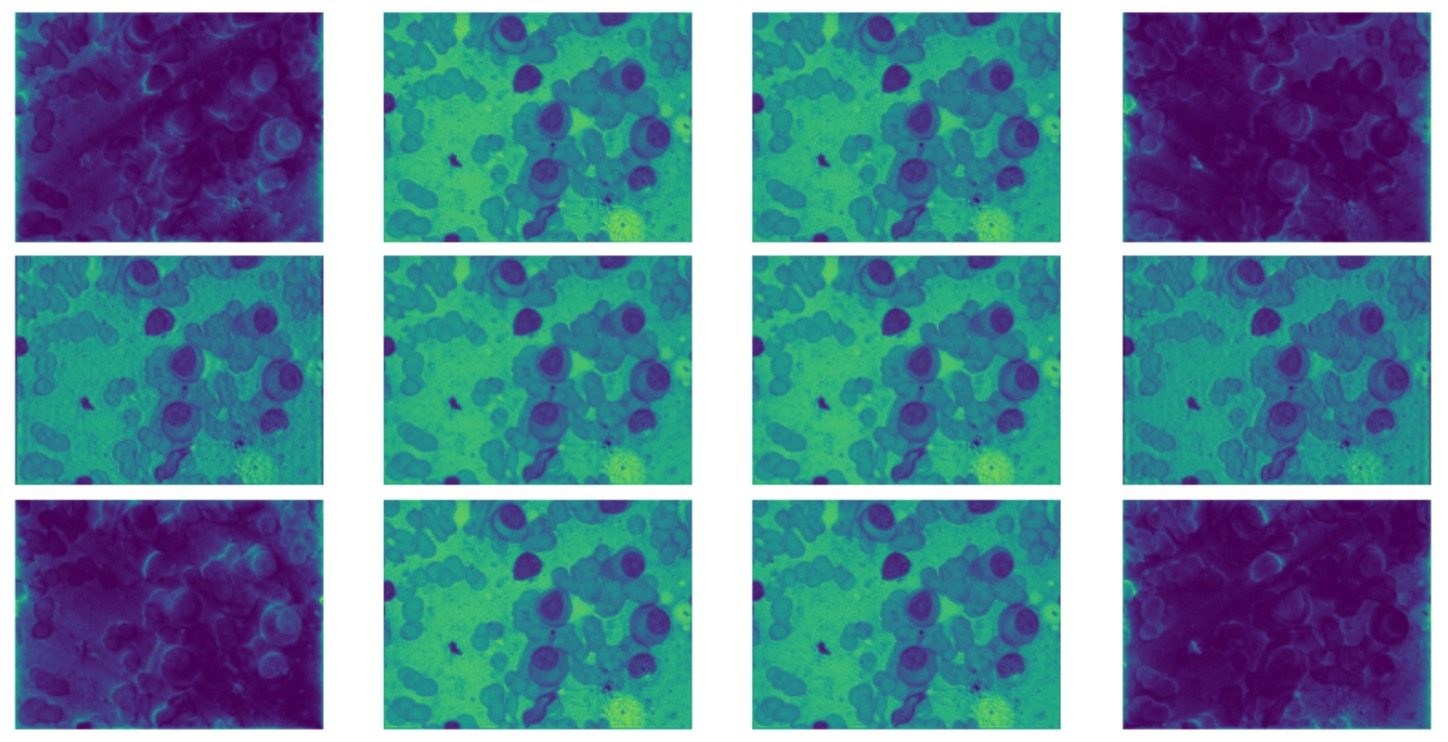
\includegraphics[width=.8\linewidth]{2.jpg}
    \captionof{figure}{Simulation of 12 light waves hitting a sample from different angles
    }
  \end{minipage}
\end{figure}

\subsubsection{Morphological Operations}

Physical image transformations, such as erosion and dilation, can significantly improve the segmentation of Multiple Myeloma cells. Erosion and dilation are morphological operations that modify the shape and size of objects within an image. Erosion is used to shrink the boundaries of objects, while dilation is used to expand them. In the context of Multiple Myeloma cell segmentation, erosion and dilation could potentially reduce or enhance, respectively, the appearance of small or spurious features in the image. Dilation may expand the boundaries of objects, making it easier to capture the entire cell and reduce the likelihood of under-segmentation. Erosion can shrink the boundaries of objects, making it easier to separate adjacent or overlapping cells and reduce the likelihood of over-segmentation. Furthermore, they help reduce noise and extract prominent features. By applying these operations to different regions of the image, it is possible to identify the size, shape, and distribution of different objects.

\subsubsection{Gradient Filters}

The gradient Sobel filter is a widely used edge detection algorithm that detects edges in an image by measuring the rate of change in pixel intensity across neighboring pixels in both the X and the Y directions. In the context of Multiple Myeloma cell segmentation, the gradient Sobel filter can be used to enhance the edges of the cells, making them more distinguishable from non-Multiple Myeloma cells. By detecting the edges of the cells, the filter can help to separate them from adjacent cells and enhance the precision of segmentation algorithms. It may further help distinguish between areas covered by the nucleus and those by the cytoplasm. Additionally, the gradient Sobel filter can be combined with other physical image transformations, such as thresholding or morphological operations, to further enhance the segmentation of Multiple Myeloma cells. For example, the filter can be used to enhance the edges of cells, followed by a thresholding operation to segment them based on pixel intensity values.

\begin{figure}
  \centering
  \begin{minipage}{.5\textwidth}
    \centering
    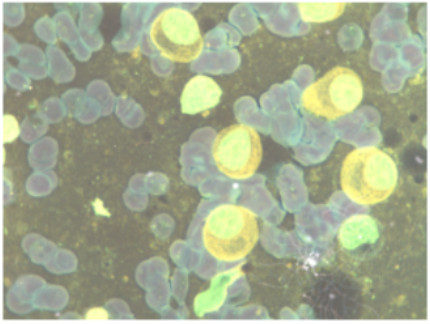
\includegraphics[width=.5\linewidth]{3.png}
    \captionof{figure}{Image after contrast normalization}
  \end{minipage}%
  \begin{minipage}{.4\textwidth}
    \centering
    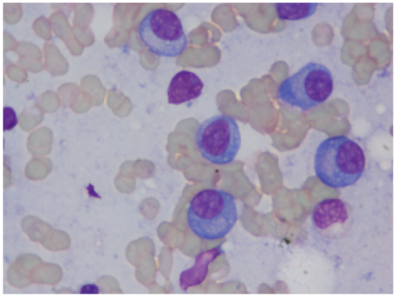
\includegraphics[width=.63\linewidth]{4.png}
    \captionof{figure}{Image after Dilation operation}
  \end{minipage}
\end{figure}

\subsubsection{Manipulating Color Channels}

Color channel enhancement involves increasing the contrast and brightness of a specific color channel (Red, Green, or Blue) while keeping the others unchanged. In the context of Multiple Myeloma cell segmentation, this technique can help to improve the contrast and visibility of stained cells by enhancing the color channel that provides the most information about the cells. For example, Multiple Myeloma cells may have a different color or hue than non-Multiple Myeloma cells in the image. By enhancing the color channel that represents this difference, the cells can become more visible and distinguishable in the image.

\begin{figure}
  \centering
  \begin{minipage}{.5\textwidth}
    \centering
    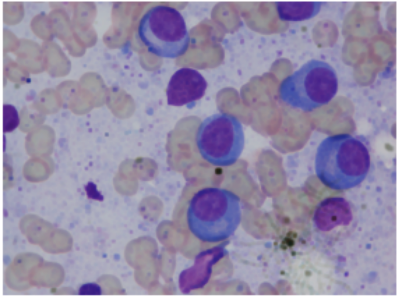
\includegraphics[width=.5\linewidth]{5.png}
    \captionof{figure}{Image after Erosion operation}
  \end{minipage}%
  \begin{minipage}{.4\textwidth}
    \centering
    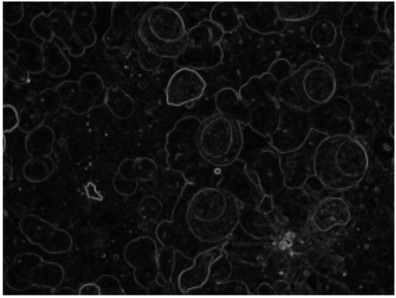
\includegraphics[width=.63\linewidth]{6.png}
    \captionof{figure}{Image after Sobel filter}
  \end{minipage}
\end{figure}
\subsubsection{Blur Filters}

Applying a Gaussian or Median blur to an image can improve the segmentation of Multiple Myeloma cells by reducing the impact of noise and enhancing the edges of the cells. Both techniques involve smoothing the image by replacing each pixel's value with the average of surrounding pixels'. Gaussian blur works by convolving the image with a Gaussian kernel, which gives more weight to pixels closer to the center of the kernel. This has the effect of blurring the image while preserving the edges and details of the objects in the image. Median blur works by replacing each pixel's value with the median value of surrounding pixels, which can help to remove small, random fluctuations in pixel values. Noise can make it difficult to accurately detect the edges and boundaries of the cells, leading to segmentation errors. By smoothing the image with a blur filter, we can reduce the impact of noise and make it easier to detect the edges of the cells.

\begin{figure}
  \centering
  \begin{minipage}{1\textwidth}
    \centering
    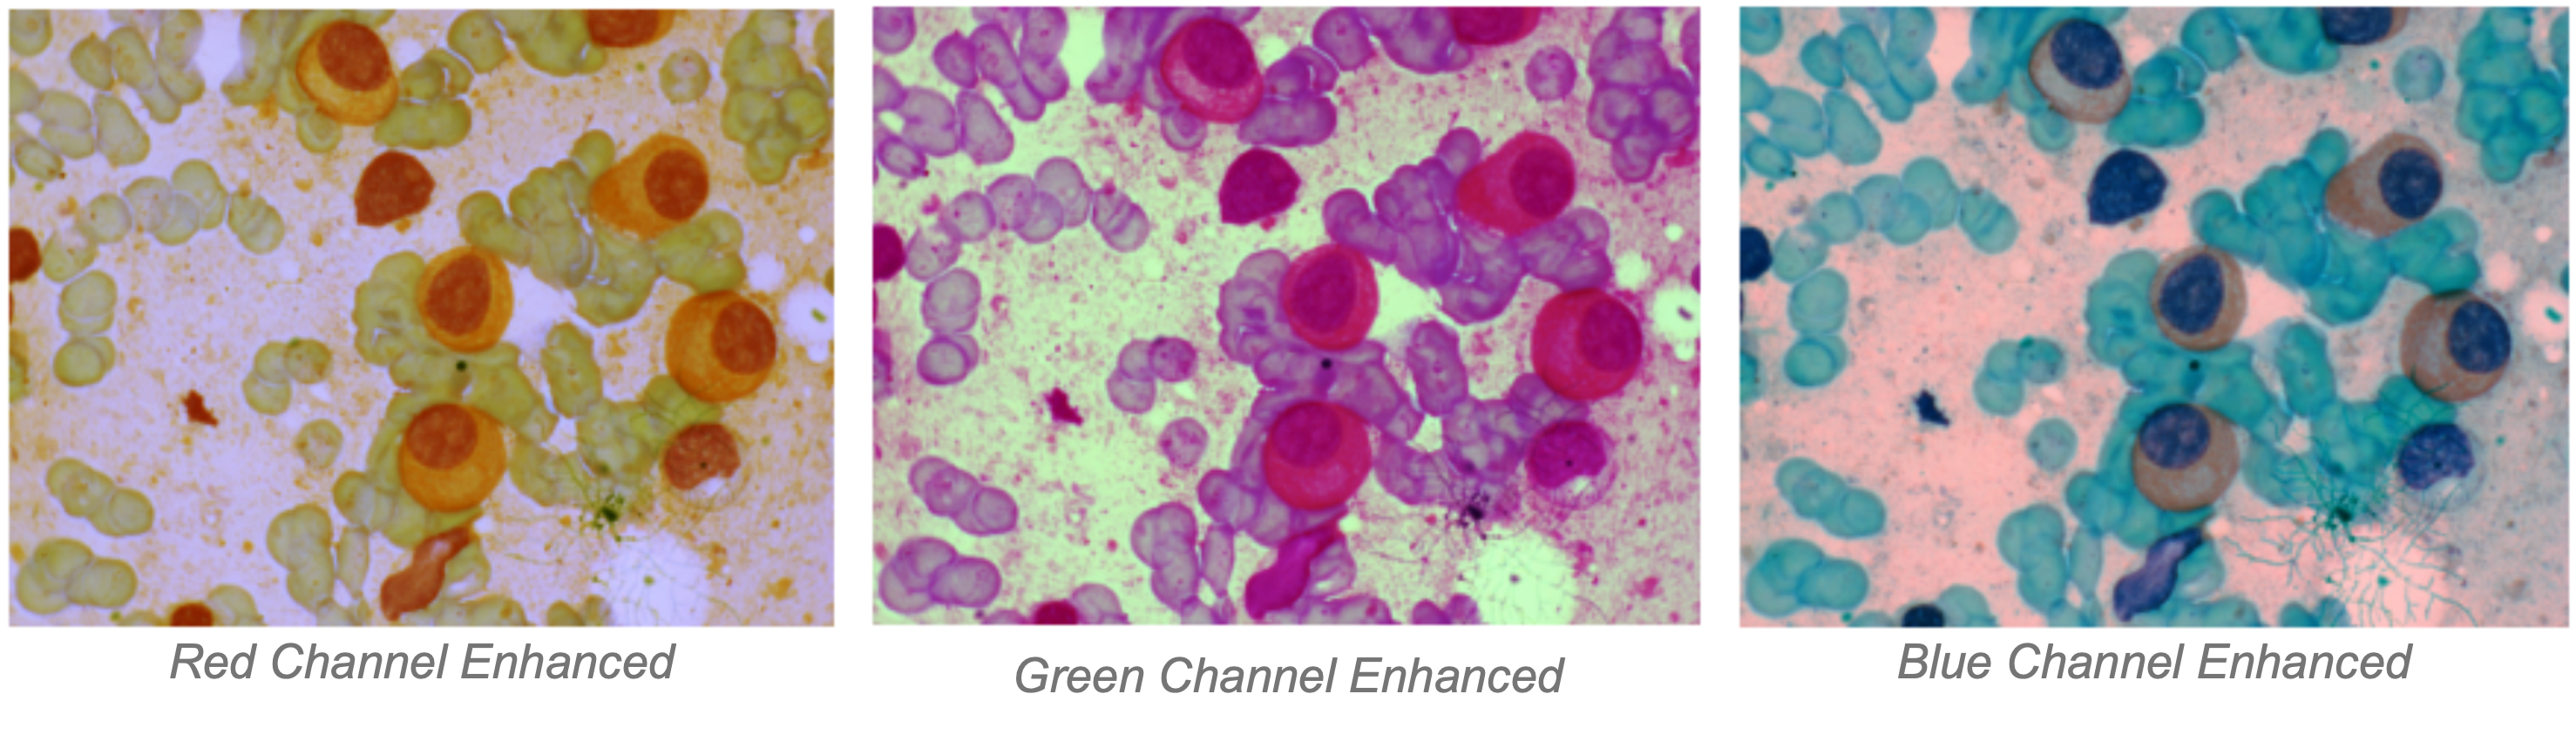
\includegraphics[width=0.8\linewidth]{7.png}
    \captionof{figure}{Image after applying color channel enhancement}
  \end{minipage}%
\end{figure}

\begin{figure}
  \centering
  \begin{minipage}{.5\textwidth}
    \centering
    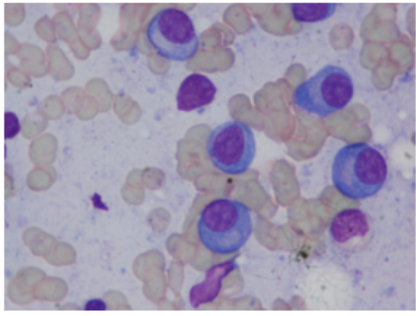
\includegraphics[width=.5\linewidth]{8.png}
    \captionof{figure}{Image after Gaussian Blur}
  \end{minipage}%
  \begin{minipage}{.4\textwidth}
    \centering
    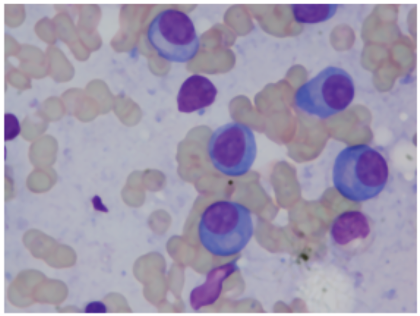
\includegraphics[width=.63\linewidth]{9.png}
    \captionof{figure}{Image after Median Blur}
  \end{minipage}
\end{figure}

\begin{table}[b]
  \caption{Performance comparison of the 11 models on the validation and test sets}
  \label{sample-table}
  \centering
  \begin{tabular}{lccc}
    \toprule
    \multicolumn{2}{c}{ }\\
    {\bf Image} & {\bf Nucleus Segmentation} & {\bf Cytoplasm Segmentation} & {\bf Test} \\
    {\bf Transformation} & {\bf Validation AP} & {\bf Validation AP} & {\bf Mean IOU}   \\
    \midrule
    None & 80.39 & 44.34 & 0.85 \\
    \midrule
    Illumination Simulation & 77.64 & 41.46 & 0.84 \\
    \midrule
    Contrast Normalization & 78.21 & 44.05 & 0.84 \\
    \midrule
    Erosion & 78.76 & 43.83 & 0.84 \\
    \midrule
    Dilation & {\bf 82.00} & 43.79 & 0.85 \\
    \midrule
    Sobel Gradient Filter & 74.13 & 38.53 & 0.83 \\
    \midrule
    Red Channel Enhancement & 79.87 & 42.97 & 0.85 \\
    \midrule
    Green Channel Enhancement & 79.91 & 42.32 & 0.86 \\
    \midrule
    Blue Channel Enhancement & 79.04 & 43.51 & 0.85 \\
    \midrule
    Gaussian Blur Filter & 81.74 & 43.95 & 0.84 \\
    \midrule
    Median Blur Filter & 81.52 & {\bf 46.03} & {\bf 0.87} \\
   \bottomrule
 \end{tabular}
\end{table}

\begin{figure}
  \centering
  \begin{minipage}{1\textwidth}
    \centering
    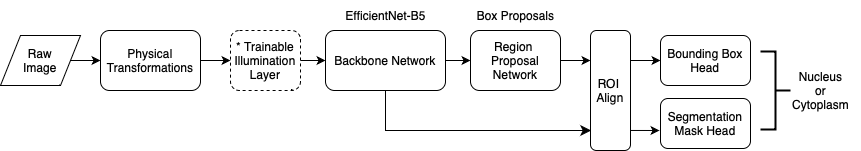
\includegraphics[width=1\linewidth]{10.png}
    \captionof{figure}{Machine Learning Pipeline \emph{(*trainable layer exists only in illumination simulation case)}}
  \end{minipage}%
\end{figure}

\subsection{Machine Learning Model}

A Mask R-CNN model was used to perform instance segmentation of Multiple Myeloma cell nucleus and cytoplasm. The model was implemented using the PyTorch deep learning framework and the Detectron2 library. It consisted of a backbone network, a Region Proposal Network (RPN) and two Mask Heads. The backbone network was used to extract features from the input image, which were then fed to the RPN to generate region proposals. The Mask Heads were used to predict the nucleus segmentation and cytoplasm segmentation masks for each region proposal. EfficientNet B5 [6] was chosen as the backbone network. In the case of illumination simulation, an additional non-negative convolutional layer was added to convolve the illuminated images prior to being passed to EfficientNet. The selection of this non-negative attribute was a conscious choice as it is illogical for illumination weights to bear negative values in real life. The outputs of the model were the predicted probability scores of nucleus segmentation mask and cytoplasm segmentation mask. The model was trained for a total of 3725 steps with a learning rate of 0.0025 and a Warmup Cosine Learning Rate scheduler. Training was done on a single NVIDIA RTXA6000 GPU with 48GB of memory. The model was trained on the train set and evaluated on the validation set. The model with the best validation loss was selected for submission to the SEG-PC 2021 challenge website to obtain the Mean IOU score on the test set. A total of 11 models were trained, among which were 10 that incorporated one of the aforementioned physical image transformations and 1 that did not have any transformation.

\section{Results}

The metric for comparing our models with different physical transformations is the Average Precision (AP). It is calculated by plotting precision against recall and taking the area under the curve (AUC). A higher AP indicates better performance, with a maximum value of 1.0 indicating perfect precision and recall. The best performance in nucleus segmentation was achieved by applying morphological transformation like dilation, which expanded the boundaries of cell nuclei, making it easier to capture them and reducing the likelihood of under- or non-segmentation. In the case of cytoplasm segmentation, the Median Blur filter delivered the best performance. This reduced the impact of noise and enhanced the edges of Multiple Myeloma cells and their nuclei resulting in the model being able to better identify the area covered by the cytoplasm. We submitted our segmentation results to the SEG-PC 2021 challenge website to benchmark our different models on the unseen test images, as their ground truth labels were not made available. In terms of overall performance across both nucleus and cytoplasm segmentations, the Medium Blur Filter attained the best Mean IOU from the test images.

\section{Conclusion}

Multiple Myeloma is a challenging and complex type of blood cancer that requires accurate identification and segmentation of plasma cells in order to aid in diagnosis, prognosis, and treatment planning. In this study, we have explored the effectiveness of various physical image transformations to improve the accuracy of Multiple Myeloma cell segmentation. Our results have shown that certain physical image transformations, such as Dilation and Median Blur filter, were effective in improving the Average Precision and Mean IOU of our baseline model. These transformations helped to enhance the contrast and reduce noise in the images, resulting in more accurate and consistent segmentation of Multiple Myeloma cells.

While the individual physical image transformations showed results similar to the baseline model without any transformation, we believe that further improvements can be achieved by combining multiple transformations in an ensemble approach. This may help to address the limitations of each individual transformation and enhance the overall performance of the segmentation model.

In conclusion, our study demonstrated the potential of physical image transformations to improve Multiple Myeloma cell segmentation. These findings can contribute to the development of more effective and reliable segmentation models for the diagnosis and treatment of Multiple Myeloma.

\begin{thebibliography}{99}

  \bibitem{} SegPC-2021 - Grand Challenge. grand-challenge.org. Accessed April 19, 2023. https://segpc-2021.grand-challenge.org
  \bibitem{} He K, Gkioxari G, Dollár P, Girshick R. Mask R-CNN. arXiv.org. Published 2017. doi: https://doi.org/10.48550/arXiv.1703.06870
  \bibitem{} Gupta A, Shiv Gehlot, Goswami S, et al. SegPC-2021: A challenge \& dataset on segmentation of Multiple Myeloma plasma cells from microscopic images. Medical Image Analysis. 2022;83:102677-102677. doi:https://doi.org/10.1016/j.media.2022.102677
  \bibitem{} Paing MP, Sento A, Bui TH, Pintavirooj C. Instance Segmentation of Multiple Myeloma Cells Using Deep-Wise Data Augmentation and Mask R-CNN. Entropy. 2022;24(1):134. doi:https://doi.org/10.3390/e24010134
  \bibitem{} Wu Y, Kirillov A, Massa F, Lo W, Girshick R. Detectron2. Published 2019. https://github.com/facebookresearch/detectron2
  \bibitem{} Tan M, Le QV. EfficientNet: Rethinking Model Scaling for Convolutional Neural Networks. arXiv.org. Published 2019. doi: https://doi.org/10.48550/arXiv.1905.11946
  
\end{thebibliography}

\end{document}